%=====================================================================
% DRAFT STATUS — REMOVE THIS BLOCK BEFORE SUBMISSION
% Draft v2 (LaTeX), 2026-08-14. Target journal: Plant Physiology.
% Based on markdown draft v1 (2026-08-13) with: verified references,
% author/funding blocks from the author list, Gate 1 strict frozen-test
% numbers inserted in R2, cohort updated to the actual 593 sites.
%
% PENDING before submission:
%   1. OSF preregistration DOI -> insert in R5, Methods, Data availability
%   2. Gate 3 blind cohort -> complete R6/R7, Table 5, Figure 6, Abstract
%      outcome sentence (two pre-written variants kept as comments)
%   3. Public archive DOI (Zenodo) for code + data archive
%   4. ORCIDs for all authors
%   5. Confirm CRediT roles with all co-authors
%
% WORDING GATE (binding): this file must pass
% verify_predictive_claims -> [] (hold decision) and
% find_forbidden_external_claims -> [] after ANY edit. Negations of
% forbidden phrases also trip the matchers; reword, never negate.
%=====================================================================
\documentclass[namedate,unnumsec,webpdf,contemporary,large]{oup-authoring-template}

\graphicspath{{figures/}}
\newcommand{\societylogo}{}

% line numbers for review
%\usepackage[mathlines,switch]{lineno}

\begin{document}

\journaltitle{Plant Physiology}
\DOI{DOI added during production}
\copyrightyear{2026}
\pubyear{2026}
\vol{XX}
\issue{x}
\access{Advance access publication date added during production}
\appnotes{Research Article}

\firstpage{1}

\title[Preregistered ranking of persulfidation candidates]{A frozen, preregistered framework for proteome-wide ranking of candidate cysteine persulfidation sites in tomato (\textit{Solanum lycopersicum})}

\author[1,2]{Guohao Lu}
\author[1,2]{Yingchun Xia}
\author[1,2]{Huichao Liu}
\author[1,2]{Xiaolei Zhu}
\author[1,2]{Shuai Yang}
\author[3,4,$\ast$]{Ailian Zhou}
\author[1,2,$\ast$]{Lichuan Gu}

\address[1]{\orgdiv{School of Artificial Intelligence}, \orgname{Anhui Agricultural University}, \orgaddress{\street{Hefei}, \postcode{230036}, \country{China}}}
\address[2]{\orgname{Anhui Province Key Laboratory of Intelligent Agricultural Technology and Equipment, Anhui Agricultural University}, \orgaddress{\street{Hefei}, \postcode{230036}, \country{China}}}
\address[3]{\orgdiv{Agricultural Information Institute}, \orgname{Chinese Academy of Agricultural Sciences}, \orgaddress{\street{Beijing}, \postcode{100081}, \country{China}}}
\address[4]{\orgname{Key Laboratory of Agricultural Blockchain Application, Ministry of Agriculture and Rural Affairs}, \orgaddress{\street{Beijing}, \postcode{100081}, \country{China}}}

\corresp[$\ast$]{Corresponding authors. \href{mailto:zhouailian@caas.cn}{zhouailian@caas.cn}; \href{mailto:glc@ahau.edu.cn}{glc@ahau.edu.cn}}

\received{Date}{0}{Year}
\revised{Date}{0}{Year}
\accepted{Date}{0}{Year}

\abstract{Protein persulfidation, the hydrogen sulfide (H$_2$S)-driven conversion of cysteine thiols to persulfides, is an emerging redox regulatory mechanism in plants, but site-level experimental mapping remains costly and low-throughput. Computational ranking of candidate sites could focus experimental effort, yet published tools are scarce, their training data are difficult to obtain or reuse, and performance claims rest almost exclusively on within-dataset splits. Here we present a transparent, preregistered alternative. We integrated a provenance-tracked, four-species dataset of 389,609 cysteine sites (2,334 experimentally supported positives) and benchmarked six models under literature-comparable random-protein splits; a gated-fusion positive-unlabeled ranker achieved the highest within-dataset macro average precision (0.386; next best 0.047), and it also led on a one-shot, homology-cluster frozen test scored under audit (bootstrap difference in pooled average precision +0.140, 95\% CI 0.118--0.170). We then froze this model, including weights, features, hyperparameters, the candidate table, matched controls, and the analysis plan, under SHA256 registration before any blind data existed, scored all 179,736 non-panel cysteine sites of the tomato reference proteome, and calibrated honest expectations against published tomato sites: previously unseen confirmed sites rank moderately above the list median but do not concentrate at the list top. A blind experimental cohort (200 candidates plus 393 matched controls) with a preregistered one-sided Fisher exact test was designed with full power tabulation. All artifacts, negative results, and exclusion ledgers are openly archived. This work establishes a reproducible, preregistered pipeline for candidate ranking in plant redox proteomics; its blind test will be reported regardless of outcome.}
% [GATE 3: insert outcome sentence before the final sentence. Variants:
%  A (success): "The preregistered blind cohort met its success criteria
%   (odds ratio X.XX, exact 95% CI [...], one-sided p = ..., N confirmed
%   candidates of K = 200), demonstrating enrichment of confirmed
%   persulfidation sites among frozen top-ranked candidates under fully
%   blinded conditions."
%  B (no success): "The preregistered blind cohort did not meet its
%   success criteria (odds ratio X.XX, exact 95% CI [...], one-sided
%   p = ...); we report the complete result, the pre-registered
%   sensitivity analyses, and the resource artifacts, which remain usable
%   for candidate organisation under the stated limitations."]

\keywords{persulfidation, hydrogen sulfide, cysteine modification, preregistration, blind validation, candidate prioritization, tomato, positive-unlabeled learning}

\keywords[Abbreviations]{AP, average precision; PU, positive-unlabeled; SAP, site-aware prioritization}

\maketitle

\section{Introduction}

Hydrogen sulfide (H$_2$S) has moved from toxic byproduct to recognized signaling molecule in plants, where it participates in stomatal movement, stress responses, autophagy, and fruit ripening \citep{aroca2015ssulfhydration,aroca2018h2s,zhang2021h2s,corpas2021modus}. Its best-characterized molecular mechanism is persulfidation (S-sulfhydration): the covalent conversion of reactive cysteine thiols to persulfides, which alters the activity, localization, or interactions of target proteins \citep{aroca2017persulfidation}. Site-resolved mapping of persulfidation relies on mass-spectrometric chemoproteomics, and each candidate site then requires individual experimental confirmation, a costly bottleneck that limits the field to a few large datasets in Arabidopsis \citep{aroca2017persulfidation,jurado2021nitrogen}, rice \citep{lin2026rice}, the fungal pathogen \textit{Magnaporthe oryzae} \citep{hu2025magnaporthe}, and, notably for this work, tomato, where a persulfidome linked to fruit ripening was reported by \citet{zhang2024kiae271} (hereafter ``kiae271'').

Computational prioritization of candidate sites is an attractive complement, but the available tooling is thin. Sul-BertGRU \citep{wei2025sulbertgru} is the only published persulfidation-specific deep-learning tool with retrievable training data, and our audit of that data found substantial label problems (1,003 of 2,705 entries have a non-cysteine center residue; 78\% human and 21\% Arabidopsis sequences; audit ledger in the project archive). The training data of pCysMod \citep{li2021pcysmod} could not be obtained, and iCysMod \citep{wang2021icysmod} is a database rather than a site-ranking tool. No new persulfidation-specific ranking tools appeared in the 2025 literature as of our audit date. More fundamentally, performance claims across the cysteine-PTM tool literature rest on within-dataset random splits, and blinded, preregistered experimental evaluation is essentially absent \citep{nosek2018preregistration,chambers2013registered}.

We take the position that the correct response to this situation is not a larger claim but a stricter protocol. In prior work on Arabidopsis we showed that a sequence+structure positive-unlabeled (PU) ranker carries a real but modest within-dataset signal (leave-study-out pooled AP 0.102, 2.1$\times$ base rate; both studies from one laboratory), and we froze a binding limitation statement that governs all outward text from this project:

\begin{quote}
Current public data are insufficient to demonstrate cross-study predictive ability; the model is used only for candidate organisation and hypothesis generation.
\end{quote}

Accordingly, everything in the present paper is organized around a candidate-organisation tool whose value is decided by a preregistered blind experiment, not by retrospective metrics.

Here we report: (i) a provenance-tracked, four-species site-level dataset and a literature-comparable within-dataset benchmark in which a gated-fusion PU ranker leads six models; (ii) a fully frozen, hash-registered candidate release for the tomato proteome, comprising model weights, feature schema, inference script, ranked candidate table, and matched controls; (iii) a one-shot strict-track frozen test, scored under audit, whose claim class is decided by a preregistered statistical gate; (iv) a pre-blind calibration against published tomato and Arabidopsis sites that sets honest expectations for the blind test; and (v) the preregistered blind-cohort design, power analysis, and statistical analysis plan, co-signed by the modeling and wet-laboratory partners on 2026-08-13 (preregistration DOI to be inserted at submission). The blind-cohort result will be added to this manuscript and reported regardless of outcome. All negative results, exclusions, and intermediate artifacts are preserved in a public data archive.

\section{Results}

\subsection{A provenance-tracked, four-species site-level persulfidation dataset}

We integrated site-level persulfidation evidence from four public studies into a single development panel in which each row is one cysteine site with full study provenance (accession, coordinate, label, source study): PXD006140 and PXD024061 (Arabidopsis; same laboratory and chemistry) \citep{aroca2017persulfidation,jurado2021nitrogen}, PXD072089 (rice; independent laboratory) \citep{lin2026rice}, PXD063170 (\textit{M. oryzae}) \citep{hu2025magnaporthe}, and the kiae271 tomato sites \citep{zhang2024kiae271}. The release training panel, defined as the union of the ten seed panels used for the literature-comparable benchmark (development split only; the strict-track frozen test partition was never touched), comprises 389,609 sites with 2,334 positives (SHA256 \texttt{30e432fb...}; Table~\ref{tab:scans} gives the per-species candidate-scan accounting; per-species positive counts in Supplemental Table S1). The panel is dominated by unlabeled sites (the PU learning setting \citep{elkan2008pu}): experimentally supported positives are certain, but the unlabeled pool mixes true negatives with sites never assayed.

Two provenance facts shape everything downstream and are stated up front. First, the Arabidopsis positives come from one laboratory with one chemistry; no amount of modeling converts them into cross-study evidence. Second, all 79 tomato positives in the panel are the kiae271 published sites (verified by direct key overlap; see the calibration section below): the model has seen every published tomato site there is.

\subsection{Within-dataset benchmark under literature-comparable splits}

We benchmarked six models on the integrated dataset under the split protocol customary in the cysteine-PTM tool literature (random protein-level holdout, 10 seeds): the gated-fusion PU ranker (\texttt{structure\_ranker}), an ESM-2 linear head \citep{lin2023esm2}, XGBoost, a PU logistic baseline, random forest, and a retrained Sul-BertGRU \citep{wei2025sulbertgru}. The reported metric is macro average precision (AP) averaged over the three crop species (Arabidopsis, rice, tomato). This is a within-dataset evaluation; per the project's claim gate it supports exactly one claim class, quoted verbatim:

\begin{quote}
Literature-comparable within-dataset performance improvement.
\end{quote}

\texttt{structure\_ranker} achieved mean macro AP 0.386 $\pm$ 0.173 (10 seeds), 7.9$\times$ the mean of the best-per-seed baseline and leading on every seed (Table~\ref{tab:benchmark}; Fig.~\ref{fig:benchmark}). Per-species APs were 0.493 $\pm$ 0.267 (Arabidopsis), 0.647 $\pm$ 0.257 (rice), and 0.0185 $\pm$ 0.006 (tomato): tomato is by far the hardest species within the dataset, a point we return to below.

A parallel homology-cluster-split track (5 folds; MMseqs2 clustering at 30\% identity \citep{steinegger2017mmseqs2,steinegger2018clustering}) holds a 20\% frozen test partition that was unlocked exactly once, under a hash-verified unlock procedure with a full run-manifest audit (269,801 sites, 566 positives). On this strict partition the frozen ranker scored per-species APs of 0.0996 (Arabidopsis; 125$\times$ base rate) and 0.1978 (rice; 133$\times$), against 0.0015 and 0.0023 for the strongest baseline; tomato scored 0.00032, below its own base rate (0.76$\times$) and below the baseline there, consistent with the tomato feature starvation quantified below. The preregistered cluster-bootstrap difference in pooled average precision against the strongest baseline was +0.140 (95\% CI 0.118--0.170; 10,000 replicates, seed 20260813). Because the per-species gate requires the difference to be positive in every crop species and the tomato difference was slightly negative ($-$0.0004), the preregistered statistical gate declines any stronger claim class; this result is reported as within-dataset, literature-comparable evidence only.

None of these numbers enters any external-evidence claim. Their role in this paper is to justify the choice of the model that was frozen for the blind test.

\subsection{A frozen, hash-registered candidate release for the tomato proteome}

On 2026-08-13 we froze the complete candidate release \texttt{multispecies-v2-candidate-release-v1} (Table~\ref{tab:registry}): the trained model bundle (gated fusion of three sequence features, namely local hydrophobicity, cysteine density, and local positive charge density, plus an AlphaFold structure branch \citep{jumper2021alphafold} with explicit missingness masking; ESM and study-context branches disabled; hidden width 16, dropout 0.2, 200 epochs, learning rate 0.05, 16 MC-dropout passes; training seed fixed at the freeze date, not performance-selected), the feature schema, a self-contained inference script without training code, the ranked tomato candidate table, and matched controls.

The candidate table scores 179,736 tomato cysteine sites: every cysteine of the SHA-pinned reference proteome except the 72,051 sites in the training panel. Scores span 0.0053--0.305 with an extremely flat top (the top 200 sites occupy 0.295--0.305), a direct consequence of positives being ${\sim}$0.6\% of training data (Fig.~\ref{fig:release}). A structural finding of the release: the frozen AlphaFold registry contains zero tomato accessions, so every tomato site is scored with the structure branch masked (coverage 0/179,736). Diagnostic scans with the same frozen model quantify the contrast: Arabidopsis 284,387 candidates with 1.07\% structure coverage, rice 469,748 with 0.75\% (Table~\ref{tab:scans}). Tomato ranking in this release is therefore driven entirely by the three sequence features, a feature-starvation state that the pre-blind calibration below suggests is consequential, and that any future release may address only under a new release number and a new preregistration.

For each of the top-200 candidates we pre-computed up to five matched controls (966 pairs total): non-panel tomato sites from the same structure-availability stratum, nearest by Euclidean distance in z-scored sequence-feature space, caliper 0.25 SD, no control reused (Fig.~\ref{fig:release}b). The blind analysis uses exactly the two nearest controls per candidate (rule locked at signing; the artifact itself is unchanged). Four of the 200 candidates have fewer than two controls within the frozen caliper (three with zero, one with one); these feature-extreme sites remain in the candidate arm, and the assayed cohort therefore comprises 200 candidates and 393 controls (593 sites), as recorded in the co-signed analysis plan.

\subsection{Pre-blind calibration: what published sites say to expect}

Before any blind data existed, we scored the 99 coordinate-verified kiae271 sites with the frozen bundle and ranked them within the frozen candidate table, a mock-blind diagnostic registered in advance as expectation-setting only, with results reported regardless of direction. Three facts emerged (Fig.~\ref{fig:calibration}).

First, a contamination fact: 79 of the 99 published sites are in the release training panel (100\% of the panel's tomato positives). They cannot inform expectations and are excluded from interpretation. Second, the clean subset: the 20 sites the model never saw rank moderately high, with 13/20 (65\%) above the candidate-table median (mean percentile 60.5; two-sided binomial against 50\% $p = 0.26$). Third, the decisive observation: 0 of 99 published sites appear in the candidate table's top 2,000.

The same pattern repeats on seven Arabidopsis control sites from laboratories independent of all training data (DES1, RBOHD, SnRK2.6/OST1, ABI4, ATG4a, AtG6PD6, and PAD3 \citep{zhang2026pad3}; all coordinate-verified against the v2 proteome): 5/7 above the median (mean percentile 56.7, range 4.9--85.8; two-sided $p = 0.45$).

Our reading, stated before unblinding: the frozen model carries a genuine but mild mid-list ranking signal, and true sites do not concentrate at the list top. The blind Top-K enrichment we consider plausible a priori is modest (odds ratio on the order of 1.5--2.5), which directly motivates the large-K design below. This calibration is registered with full per-site data in the project archive; it changes nothing in the frozen artifacts, and it prevents the field (and us) from over-reading the blind outcome in either direction.

\subsection{Preregistered blind-cohort design and statistical analysis plan}

The blind validation is fixed in two co-signed documents, the Site-Aware Prioritization (SAP) protocol and the analysis plan (\texttt{sap\_protocol.json}, \texttt{analysis\_plan.json} in the release package; preregistration DOI to be inserted at submission). Core elements:

\begin{itemize}
\item \textbf{Cohort.} Top-200 candidates from the frozen table plus 393 matched controls (593 sites), assayed blind by the wet-laboratory partner; labels remain with the wet laboratory until the preregistered unblinding step. Sites on proteins carrying published kiae271 persulfidation are excluded from the primary analysis and retained only as a preregistered sensitivity stratum; process controls are defined by the wet laboratory before measurement.
\item \textbf{Primary endpoint.} Enrichment of experimentally confirmed persulfidation sites among Top-200 candidates relative to matched controls; one-sided Fisher exact test ($\alpha = 0.05$, preregistered direction) with odds ratio and exact 95\% CI. Success criteria: $p < 0.05$ and OR $> 1$ and at least 2 confirmed candidate sites.
\item \textbf{Design and power.} Because the effect size is unknowable before blind data exist, power was tabulated over the full grid $K \in \{50,100,200,300\}$ $\times$ controls-per-candidate $\in \{1,2,5\}$ $\times$ background confirmation rate $\in \{1\%,2\%,5\%\}$ $\times$ assumed OR $\in \{1.5,2,3,5\}$ (10,000 simulations per cell, seed 20260813; complete 144-cell table in \texttt{power\_table.json}). Structurally, at fixed assay budget a larger $K$ with fewer controls dominates (Fig.~\ref{fig:power}). The decided design is $K = 200$ with 2 controls per candidate (nominally 600, actually 593 assayed sites): at 2\% background rate, power 0.305 / 0.677 / 0.978 at OR 2 / 3 / 5 (Table~\ref{tab:power}). If throughput allows ${\geq}$ 900 sites, $K = 300$ raises OR = 3 power to 0.850. The minimum-viable 400-site design ($K = 200$, 1:1) is an honest coin flip at OR = 3 (power 0.524) and is flagged as such. $K$ and the control ratio are fixed before unblinding as the largest assayable design; the full power table is reported, not filtered to favorable rows.
\item \textbf{Unblinding procedure.} Two independent persons verify the bundle, fit-manifest, candidate-table, control-table, and inference-script hashes; the blind-cohort scoring output is written and hash-locked before labels are released; the preregistered analysis then runs verbatim. Forbidden after unblinding: any model, feature, Top-K, or threshold change; adding samples to a failing endpoint; re-ordering the candidate table.
\item \textbf{Reporting.} The primary analysis is reported regardless of outcome; all negative results and exclusions are preserved with provenance; any deviation requires a dated, hashed, co-signed amendment.
\end{itemize}

%=====================================================================
% GATE 3 PLACEHOLDER — DO NOT EDIT ANYTHING ABOVE THIS COMMENT AFTER
% UNBLINDING. The two sections below are completed verbatim from the
% preregistered analysis output.
%=====================================================================
\subsection{Blind-cohort primary endpoint}
\textbf{[TO BE COMPLETED AT GATE 3]} Insert verbatim: the $2\times2$ table (Table~\ref{tab:primary}), Fisher exact $p$, odds ratio with exact 95\% CI, per-endpoint numbers, and the process-control pass rate. The abstract outcome sentence is pre-written in two variants (see source comments).

\subsection{Sensitivity and secondary analyses}
\textbf{[TO BE COMPLETED AT GATE 3]} Preregistered list: (i) exclusion of any site on a training-panel protein; (ii) exclusion of kiae271-protein sites; (iii) leave-one-out over candidate proteins and over homology clusters; (iv) rank-percentile calibration of confirmed sites (Kolmogorov--Smirnov and percentile bootstrap); (v) MC-dropout uncertainty stratification; (vi) per-structure-stratum analysis, noting that no tomato structure stratum exists in this release, so (vi) is vacuous here and is retained for release-lineage completeness.

\subsection{Mechanism follow-up}
\textbf{[OPTIONAL, Gate 4]} If at least one confirmed blind hit is carried to a mechanism chain (site confirmation, Cys-to-Ser/Ala substitution, functional effect, plant phenotype, rescue), it will be reported here. Absence of this section does not affect the primary claim; its presence upgrades the journal path per the preregistered decision matrix.

\section{Discussion}

This paper does three things that, together, we believe the cysteine-PTM field currently lacks: it freezes everything before the experiment, it calibrates expectations honestly before unblinding, and it commits to publishing the blind outcome either way.

\textbf{The within-dataset signal is real but its meaning is bounded.} Under literature-comparable splits the gated-fusion PU ranker leads five alternatives by a wide margin (macro AP 0.386 vs ${\leq}$ 0.047), and its per-species pattern (Arabidopsis 0.49, rice 0.65, tomato 0.019) is itself informative: performance tracks the availability of training positives and structure features per species, not any intrinsic learnability of the modification. Tomato combines the fewest positives (79, all from one paper) with zero structure coverage and yields near-baseline within-dataset AP; on the one-shot strict frozen test its AP fell below the base rate, and the preregistered claim gate accordingly refused any stronger claim class. The model nonetheless ranks previously unseen confirmed tomato sites moderately above the list median, consistent with a weak but real sequence-context signal. We deliberately make no claim beyond these within-dataset statements; the mandated limitation quoted in the Introduction applies to every number in this paper.

\textbf{Calibration before unblinding is the contribution other fields call registered reporting.} The mock-blind diagnostic told us, before any blind data existed, that the enrichment to expect is modest (prior OR ${\sim}$ 1.5--2.5) and that success criteria built on list-top concentration would be self-deceiving. The consequence was not to tune the model, a path closed by the freeze, but to size the experiment for a modest effect (large $K$, few controls per candidate) and to pre-commit to success criteria that a modest effect can actually meet or honestly fail \citep{nosek2018preregistration,chambers2013registered}. We suggest this two-step, calibrating on published sites and then sizing the blind design, is reusable for any candidate-ranking tool in low-data proteomics.

\textbf{Limitations.} (i) All training positives trace to four studies, two of them same-laboratory Arabidopsis; the dataset cannot support cross-study statements, and none are made. (ii) Tomato structure coverage is 0\%; the structure branch, which contributes within-dataset value for Arabidopsis and rice, is inert for tomato, and the ranking rests on three sequence features. (iii) The flat score distribution (top-200 within 0.01 score units) means rank order at the very top is fragile to small perturbations; we mitigate by reporting enrichment over $K = 200$--300 rather than any small top-N. (iv) MC-dropout uncertainty is deterministic per device but not bit-identical across CPU and GPU (different random-number streams); point scores are bit-identical. (v) The matched-control design controls sequence-feature strata, not expression, localization, or assay detectability; residual confounding by detectability cannot be excluded and is why process controls are part of the primary report. (vi) A blind failure would not falsify persulfidation biology; it would bound the usefulness of this feature set for this species, which is itself the published answer this design guarantees.

\textbf{What happens next is already written down.} Per the preregistered decision matrix: blind success plus a complete mechanism chain upgrades the submission target; blind success without mechanism stands as a resource and validation report; blind failure with intact resources stands as the same, with the negative result as a first-class finding. No model development is permitted to rescue a failed endpoint; any improved model (for example with tomato structure coverage, recalibrated scores, or expanded training positives, all registered in the project's deferred-improvement register) requires a new release number and a new preregistration.

\section{Materials and Methods}

\subsection{Dataset assembly and provenance}

Site-level positives and unlabeled cysteine pools were integrated from PXD006140 and PXD024061 (Arabidopsis) \citep{aroca2017persulfidation,jurado2021nitrogen}, PXD072089 (rice) \citep{lin2026rice}, PXD063170 (\textit{M. oryzae}) \citep{hu2025magnaporthe}, and kiae271 (tomato) \citep{zhang2024kiae271} into the multispecies v2 dataset with per-row study provenance; coordinates were verified against SHA-pinned reference proteomes (tomato reference proteome SHA256 \texttt{1a46efe6...}). The release training panel (389,609 rows, 2,334 positives; SHA256 \texttt{30e432fb...}) is the union of the ten literature-random-track seed panels, development split only. The exclusion ledger (8 entries) and the full input inventory (243 files with SHA256) are in the data archive.

\subsection{Features}

Per-site input features: three sequence-window features (local hydrophobicity, cysteine density, local positive charge density; exact definitions frozen in \texttt{feature\_schema.json}) and two AlphaFold-derived structure features \citep{jumper2021alphafold} (contact proxy, pLDDT) with an explicit availability mask; missing structures are masked, never mean-imputed. ESM-2 embeddings \citep{lin2023esm2} and study-context features are implemented but disabled in this release (\texttt{use\_esm = 0}, \texttt{use\_study\_context = false}).

\subsection{Model and training}

\texttt{structure\_ranker} is a gated-fusion PU ranker (branch encoders with gated combination; PU objective \citep{elkan2008pu}). Frozen hyperparameters: hidden width 16, dropout 0.2, 200 epochs, learning rate 0.05, holdout fraction 0.2, 16 MC-dropout passes for uncertainty. The model was trained once on the full panel with seed 20260813 (the freeze date; not performance-selected) on CUDA and serialized as \texttt{StructureRankerBundle} (PyTorch, pickle protocol 4, atomic write; SHA256 \texttt{ab8a0353...}). Point scores are bit-identical across CPU and GPU; MC-dropout uncertainty is deterministic per device. Code revision \texttt{d0c740c...} (full hash in \texttt{fit\_manifest.json}).

\subsection{Benchmark protocols}

The literature-comparable track used random protein-level holdout with 10 seeds and 6 models; the metric is macro AP across the three crop species (scripts and manifests in \texttt{results/experiments/multispecies\_v2\_global\_clusters\_v11/}). The strict track used 5-fold homology-cluster development splits (MMseqs2, 30\% identity \citep{steinegger2017mmseqs2,steinegger2018clustering}) with a 20\% frozen test partition locked under a hash-verified unlock procedure (\texttt{scripts/score\_v2\_frozen\_test.py} with a dated unlock record binding the config SHA256, code revision, and split SHA256) and a full run-manifest audit (training log, per-arm checkpoints, artifact hash re-verification). The frozen test was scored exactly once per the unlock record; the preregistered statistics are a cluster bootstrap (10,000 replicates, seed 20260813) of the pooled-primary difference in average precision against the strongest baseline, with the homology-robust claim upgrade requiring a positive bootstrap lower bound and a positive difference in every crop species.

\subsection{Candidate table and matched controls}

\texttt{scripts/generate\_tomato\_topk\_candidates.py} verifies the config against the frozen manifest, rebuilds and hash-verifies the training panel, scans every cysteine of the tomato reference proteome, drops panel sites, extracts features, scores with the frozen bundle, and writes the ranked table (179,736 rows; SHA256 \texttt{36963c71...}) plus matched controls (top-200 head; at most 5 controls per candidate; same structure-availability stratum; z-scored sequence-feature Euclidean distance; caliper 0.25 SD; no reuse; 966 pairs; SHA256 \texttt{c1752b07...}). Arabidopsis and rice diagnostic scans used the identical script with species-specific proteomes.

\subsection{Pre-blind calibration}

kiae271 sites (99 coordinate-verified) and 7 registered Arabidopsis independent-laboratory controls were scored with the frozen bundle and ranked by percentile within the respective frozen candidate tables (scripts \texttt{evaluate\_kiae271\_with\_release\_bundle.py}, \texttt{evaluate\_arabidopsis\_controls\_with\_release\_bundle.py}); two-sided binomial tests against the 50th percentile; panel overlap computed by exact key match. Per-site results are in the project archive (\texttt{results/known\_controls/}).

\subsection{Blind-cohort statistics and power analysis}

The primary test is a one-sided Fisher exact test on the $2\times2$ (candidate/control $\times$ confirmed/not-confirmed) table, with the odds ratio and exact 95\% CI at $\alpha = 0.05$. Power was estimated by Monte-Carlo simulation (10,000 replicates per cell, seed 20260813) over the 144-cell grid described in Results (\texttt{scripts/compute\_release\_power\_table.py}; \texttt{power\_table.json}). Secondary analyses: Kolmogorov--Smirnov and percentile-bootstrap rank calibration; MC-dropout uncertainty stratification (exploratory); leave-one-out sensitivity at protein and homology-cluster level.

\subsection{Reproducibility and wording governance}

All frozen artifacts carry SHA256 sums (\texttt{SHA256SUMS}, \texttt{manifest.json}); \texttt{scripts/audit\_candidate\_release.py} re-verifies hashes, bundle determinism, document signatures, and wording-gate compliance in one pass. The environment lock (\texttt{pip freeze}) and reproduction command index are in the data archive. All outward text of this project, this manuscript included, must pass the project's automated wording gate before release. The preregistration record (SAP protocol and analysis plan, co-signed versions) is deposited with the Open Science Framework (DOI to be inserted at submission).

\section{Data and code availability}

Frozen release package: \texttt{results/candidates/multispecies\_v2\_candidate\_release\_v1/} (Table~\ref{tab:registry} hashes). Data archive (inventories, exclusion ledger, negative-results register, environment lock): \texttt{results/data\_archive/nc\_entry\_gates/}. Code repository and permanent DOI (Zenodo) to be inserted at submission; the frozen state is pinned by the annotated git tag \texttt{gate0-release-v1-20260813}. Preregistration DOI to be inserted at submission. Proteomics data: PXD006140, PXD024061, PXD072089, PXD063170 (ProteomeXchange); kiae271 \citep{zhang2024kiae271}.

\section{Author contributions}
% [CONFIRM WITH ALL CO-AUTHORS BEFORE SUBMISSION]
G.L.: conceptualization, methodology, software, formal analysis, data curation, visualization, writing -- original draft. Y.X.: data curation, validation, writing -- review and editing. H.L.: data curation, investigation, writing -- review and editing. X.Z.: methodology, writing -- review and editing. S.Y.: validation, writing -- review and editing. A.Z.: supervision, funding acquisition, writing -- review and editing. L.G.: supervision, project administration, funding acquisition, writing -- review and editing.

\section{Funding}

This work was supported by the National Natural Science Foundation of China (32472007, 62301006, and 62301008), the Natural Science Foundation of Anhui Province (2308085MF217 and 2308085QF202), and the Anhui Province Key Laboratory of Intelligent Agricultural Technology and Equipment.

\section{Conflict of interest}

The authors declare no conflict of interest.

\section{Acknowledgements}

We thank the Zhang Hua laboratory (South China Agricultural University) for co-signing the preregistered protocol and for conducting the blind-cohort assays, and the laboratories who deposited the public persulfidome datasets used here.

\begin{thebibliography}{10}

\bibitem[Aroca et al.(2015)]{aroca2015ssulfhydration}
Aroca Á, Serna A, Gotor C, Romero LC.
\newblock S-sulfhydration: a cysteine posttranslational modification in plant systems.
\newblock {\em Plant Physiol}, 168: 334--342, 2015. doi:10.1104/pp.15.00009.

\bibitem[Aroca et al.(2017)]{aroca2017persulfidation}
Aroca Á, Benito JM, Gotor C, Romero LC.
\newblock Persulfidation proteome reveals the regulation of protein function by hydrogen sulfide in diverse biological processes in Arabidopsis.
\newblock {\em J Exp Bot}, 68: 4915--4927, 2017. doi:10.1093/jxb/erx294.

\bibitem[Aroca et al.(2018)]{aroca2018h2s}
Aroca Á, Gotor C, Romero LC.
\newblock Hydrogen sulfide signaling in plants: emerging roles of protein persulfidation.
\newblock {\em Front Plant Sci}, 9: 1369, 2018. doi:10.3389/fpls.2018.01369.

\bibitem[Chambers(2013)]{chambers2013registered}
Chambers CD.
\newblock Registered Reports: a new publishing initiative at Cortex.
\newblock {\em Cortex}, 49: 609--610, 2013. doi:10.1016/j.cortex.2012.12.016.

\bibitem[Corpas et al.(2021)]{corpas2021modus}
Corpas FJ, González-Gordo S, Muñoz-Vargas MA, Rodríguez-Ruiz M, Palma JM.
\newblock The modus operandi of hydrogen sulfide (H$_2$S)-dependent protein persulfidation in higher plants.
\newblock {\em Antioxidants (Basel)}, 10: 1686, 2021. doi:10.3390/antiox10111686.

\bibitem[Elkan and Noto(2008)]{elkan2008pu}
Elkan C, Noto K.
\newblock Learning classifiers from only positive and unlabeled data.
\newblock In {\em Proceedings of the 14th ACM SIGKDD International Conference on Knowledge Discovery and Data Mining}, pages 213--220, 2008. doi:10.1145/1401890.1401920.

\bibitem[Hu et al.(2025)]{hu2025magnaporthe}
Hu H, Qin M, Zhang J, Jiang J, Su Z, Guan L, et al.
\newblock H$_2$S-mediated protein S-sulfhydration modulates infectivity and autophagy in the rice blast fungus.
\newblock {\em Nat Commun}, 16: 6222, 2025. doi:10.1038/s41467-025-61582-8.

\bibitem[Jumper et al.(2021)]{jumper2021alphafold}
Jumper J, Evans R, Pritzel A, Green T, Figurnov M, Ronneberger O, et al.
\newblock Highly accurate protein structure prediction with AlphaFold.
\newblock {\em Nature}, 596: 583--589, 2021. doi:10.1038/s41586-021-03819-2.

\bibitem[Jurado-Flores et al.(2021)]{jurado2021nitrogen}
Jurado-Flores A, Romero LC, Gotor C.
\newblock Label-free quantitative proteomic analysis of nitrogen starvation in Arabidopsis root reveals new aspects of H$_2$S signaling by protein persulfidation.
\newblock {\em Antioxidants (Basel)}, 10: 508, 2021. doi:10.3390/antiox10040508.

\bibitem[Li et al.(2021)]{li2021pcysmod}
Li S, Yu K, Wu G, Zhang Q, Wang P, Zheng J, Liu Z-X, Wang J, Liu Y, Yu J.
\newblock pCysMod: prediction of multiple cysteine modifications based on deep learning framework.
\newblock {\em Front Cell Dev Biol}, 9: 617366, 2021. doi:10.3389/fcell.2021.617366.

\bibitem[Lin et al.(2023)]{lin2023esm2}
Lin Z, Akin H, Rao R, Hie B, Zhu Z, Lu W, et al.
\newblock Evolutionary-scale prediction of atomic-level protein structure with a language model.
\newblock {\em Science}, 379: 1123--1130, 2023. doi:10.1126/science.ade2574.

\bibitem[Lin et al.(2026)]{lin2026rice}
Lin Z, Zhou M, Ma X, Li M, Fu L, Li H, Liu Y, Zhu F-Y, Van Montagu M, Van Breusegem F, Huang J, Xie Y.
\newblock H$_2$S-mediated protein persulfidation regulates redox metabolic flux underlying salt-stress resilience in rice.
\newblock {\em Proc Natl Acad Sci USA}, 123: e2608150123, 2026. doi:10.1073/pnas.2608150123.

\bibitem[Nosek et al.(2018)]{nosek2018preregistration}
Nosek BA, Ebersole CR, DeHaven AC, Mellor DT.
\newblock The preregistration revolution.
\newblock {\em Proc Natl Acad Sci USA}, 115: 2600--2606, 2018. doi:10.1073/pnas.1708274114.

\bibitem[Steinegger and Söding(2017)]{steinegger2017mmseqs2}
Steinegger M, Söding J.
\newblock MMseqs2 enables sensitive protein sequence searching for the analysis of massive data sets.
\newblock {\em Nat Biotechnol}, 35: 1026--1028, 2017. doi:10.1038/nbt.3988.

\bibitem[Steinegger and Söding(2018)]{steinegger2018clustering}
Steinegger M, Söding J.
\newblock Clustering huge protein sequence sets in linear time.
\newblock {\em Nat Commun}, 9: 2542, 2018. doi:10.1038/s41467-018-04964-5.

\bibitem[Wang et al.(2021)]{wang2021icysmod}
Wang P, Zhang Q, Li S, Cheng B, Xue H, Wei Z, Shao T, Liu Z-X, Xue Y, Yu J.
\newblock iCysMod: an integrative database for protein cysteine modifications in eukaryotes.
\newblock {\em Brief Bioinform}, 22: bbaa400, 2021. doi:10.1093/bib/bbaa400.

\bibitem[Wei et al.(2025)]{wei2025sulbertgru}
Wei X, Ning Q, Che K, Liu Z, Li H, Guo S.
\newblock Sul-BertGRU: an ensemble deep learning method integrating information entropy-enhanced BERT and directional multi-GRU for S-sulfhydration sites prediction.
\newblock {\em Bioinformatics}, 41: btaf078, 2025. doi:10.1093/bioinformatics/btaf078.

\bibitem[Zhang et al.(2021)]{zhang2021h2s}
Zhang J, Zhou M, Zhou H, Zhao D, Gotor C, Romero LC, Shen J, Ge Z, Zhang Z, Shen W, Yuan X, Xie Y.
\newblock Hydrogen sulfide, a signaling molecule in plant stress responses.
\newblock {\em J Integr Plant Biol}, 63: 146--160, 2021. doi:10.1111/jipb.13022.

\bibitem[Zhang et al.(2024)]{zhang2024kiae271}
Zhang M, Hu K, Ma L, Geng M, Zhang C, Yao G, Zhang H.
\newblock Persulfidation and phosphorylation of transcription factor SlWRKY6 differentially regulate tomato fruit ripening.
\newblock {\em Plant Physiol}, 196: 210--227, 2024. doi:10.1093/plphys/kiae271.

\bibitem[Zhang et al.(2026)]{zhang2026pad3}
Zhang W, Zhang J, Bo S, Zhan L, Xue Q, Fan L, Pei Y, Jin Z.
\newblock H$_2$S-induced PAD3 persulfidation balances H$_2$S--HCN homoeostasis for osmotic stress tolerance in Arabidopsis.
\newblock {\em Plant Cell Environ}, 49: 5965--5978, 2026. doi:10.1111/pce.70593.

\end{thebibliography}

\clearpage

\section*{Tables}

\begin{table}[!htbp]
\caption{Proteome-wide candidate scans with the frozen model.}
\label{tab:scans}
\begin{tabular}{@{}llrrrr@{}}
\toprule
Species & Role & Panel sites excluded & Candidate sites & Structure-covered & Max score \\
\midrule
Tomato (\textit{S. lycopersicum}) & frozen release & 72,051 & 179,736 & 0 (0\%) & 0.3053 \\
Arabidopsis & diagnostic & 111,496 & 284,387 & 3,050 (1.07\%) & 0.3615 \\
Rice (\textit{O. sativa}) & diagnostic & 185,379 & 469,748 & 3,539 (0.75\%) & 0.3614 \\
\botrule
\end{tabular}
\end{table}

\begin{table}[!htbp]
\caption{Within-dataset literature-comparable benchmark (macro average precision over the three crop species, 10 seeds). Claim class for this table (verbatim, binding): ``Literature-comparable within-dataset performance improvement.'' These numbers are within-dataset evidence only.}
\label{tab:benchmark}
\begin{tabular}{@{}lrrrr@{}}
\toprule
Model & Mean & SD & Min & Max \\
\midrule
\texttt{structure\_ranker} & 0.386 & 0.173 & 0.166 & 0.554 \\
ESM-2 linear head & 0.047 & 0.007 & 0.037 & 0.055 \\
XGBoost & 0.036 & 0.008 & 0.030 & 0.059 \\
PU logistic & 0.035 & 0.007 & 0.028 & 0.050 \\
Random forest & 0.030 & 0.004 & 0.026 & 0.038 \\
Sul-BertGRU (retrained) & 0.021 & 0.002 & 0.018 & 0.024 \\
\botrule
\end{tabular}
\end{table}

\begin{table}[!htbp]
\caption{Frozen artifact registry (release \texttt{multispecies-v2-candidate-release-v1}, 2026-08-13).}
\label{tab:registry}
\begin{tabular}{@{}ll@{}}
\toprule
Artifact & SHA256 \\
\midrule
Model bundle (\texttt{structure\_ranker\_bundle.pt}) & \texttt{ab8a03532898726b765d3da18fe34736e7920cfed82134ec06195dc21b156cd3} \\
Fit manifest & \texttt{caf3c7f4d82b7dc88836bc2c16a48f5209ef95ac600bc0fbfc7a8722d07f8dbb} \\
Training panel (389,609 rows) & \texttt{30e432fb3c558c69e92362fb36d26abe1dee0f25bd23df417ad40886449156cd} \\
Tomato candidate table (179,736 rows) & \texttt{36963c7144792752a6d6b6e197da6c24fc0c8844d9540d8b63cf861dc7b7e949} \\
Matched controls (966 pairs) & \texttt{c1752b071e4413b17e41e4206d013c3c32759a6d7825da6cc299520abaefb404} \\
Frozen experiment config (v11) & \texttt{ed8b76bef0b201bb669322ff5610e84c42ba422aa8cf5b9eb274427325f7dbaf} \\
Tomato reference proteome & \texttt{1a46efe6461b239ec80b915a4c23ea39bbe39e37d43f9cc7c38b648523efca0f} \\
Training seed & \texttt{20260813} \\
Code revision & \texttt{d0c740cc24a0ce81157d23921f7875ea5f862606} \\
\botrule
\end{tabular}
\end{table}

\begin{table}[!htbp]
\caption{Preregistered design options and power (2\% background confirmation rate; one-sided Fisher exact test, $\alpha = 0.05$; 10,000 simulations per cell, seed 20260813). The full 144-cell grid is reported unfiltered in \texttt{power\_table.json} per the analysis plan.}
\label{tab:power}
\begin{tabular}{@{}lrrrrrr@{}}
\toprule
Design & $K$ & Controls/candidate & Total sites & Power OR = 2 & Power OR = 3 & Power OR = 5 \\
\midrule
Recommended & 200 & 2 & 600 & 0.305 & 0.677 & 0.978 \\
Escalation (if throughput allows) & 300 & 2 & 900 & --- & 0.850 & --- \\
Minimum viable & 200 & 1 & 400 & --- & 0.524 & --- \\
\botrule
\end{tabular}
\end{table}

\begin{table}[!htbp]
\caption{\textbf{[GATE 3 PLACEHOLDER]} Primary $2\times2$ table: candidates vs matched controls $\times$ confirmed/not-confirmed, with Fisher exact $p$ and odds ratio (exact 95\% CI).}
\label{tab:primary}
\begin{tabular}{@{}lrr@{}}
\toprule
Arm & Confirmed & Not confirmed \\
\midrule
Candidates ($n = 200$) & [Gate 3] & [Gate 3] \\
Matched controls ($n = 393$) & [Gate 3] & [Gate 3] \\
\botrule
\end{tabular}
\end{table}

\clearpage

\section*{Figure legends}

\begin{itemize}
\item[\textbf{Fig.~\ref{fig:pipeline}.}] \textbf{Study design and gate pipeline.} Every stage of the study is frozen or preregistered before any blind data exist: dataset assembly, within-dataset benchmark, SHA256-registered freeze with co-signature, pre-blind calibration, OSF preregistration, and the blind cohort. The binding no-backfitting rule and the preregistered decision matrix are shown below the pipeline.
\item[\textbf{Fig.~\ref{fig:benchmark}.}] \textbf{Within-dataset literature-comparable benchmark.} (a) Per-seed macro average precision (AP; mean over the three crop species) for six models under random protein-level holdout (10 seeds; dots, per-seed values; horizontal bar, mean; whiskers, $\pm$1 SD). (b) Per-species AP of the frozen ranker across seeds; dashed red lines mark each species' positive base rate. All values are within-dataset evidence.
\item[\textbf{Fig.~\ref{fig:release}.}] \textbf{Frozen tomato candidate release.} (a) Score distribution of all 179,736 candidate sites (log-scale counts); the red band marks the top 200, and the inset shows the flat score head across ranks 1--200. (b) Distance distribution of the 966 matched control--candidate pairs in z-scored sequence-feature space; the dashed line marks the frozen 0.25 SD caliper.
\item[\textbf{Fig.~\ref{fig:calibration}.}] \textbf{Pre-blind calibration against published sites.} (a) Percentile ranks of the 20 kiae271 tomato sites the frozen model never saw within the frozen tomato candidate table (blue, above median; grey, below). 79 of 99 published sites sit in the training panel and are excluded from interpretation; 0 of 99 appear in the candidate-table top 2,000. (b) Percentile ranks of 7 Arabidopsis control sites from laboratories independent of all training data. Dashed red lines mark the table median.
\item[\textbf{Fig.~\ref{fig:power}.}] \textbf{Preregistered power landscape.} Simulated power (one-sided Fisher exact test, $\alpha = 0.05$) over candidate count $K$ and assumed odds ratio at the 2\% background confirmation rate, shown for 1, 2, and 5 controls per candidate (10,000 simulations per cell, seed 20260813). The cyan frame marks the recommended $K = 200$, 2-controls design.
\item[\textbf{Figure 6.}] \textbf{[GATE 3 PLACEHOLDER] Blind-cohort result.} Confirmation rate in candidates vs matched controls with exact confidence intervals, and the rank-percentile distribution of confirmed sites.
\end{itemize}

\clearpage

\begin{figure}[!htbp]
\center{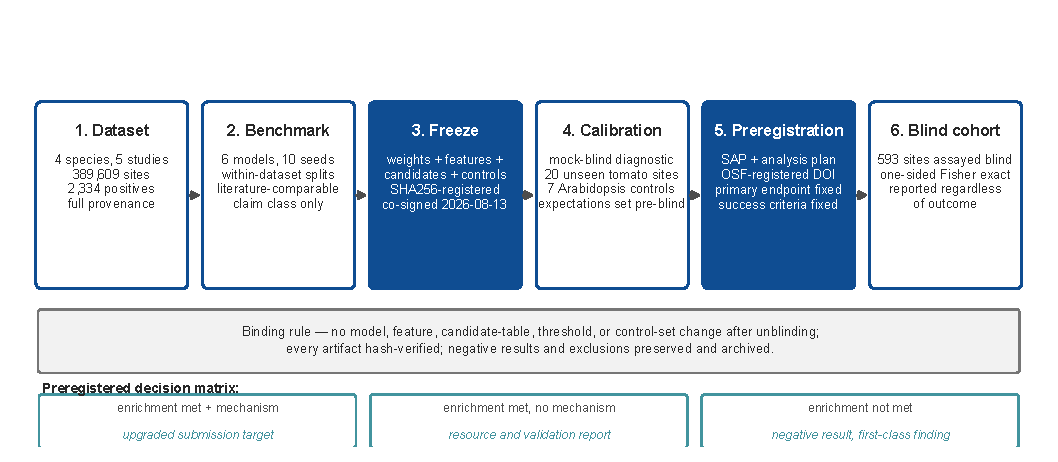
\includegraphics[width=\textwidth]{fig1_design_pipeline.pdf}}
\caption{Study design and gate pipeline.}
\label{fig:pipeline}
\end{figure}

\begin{figure}[!htbp]
\center{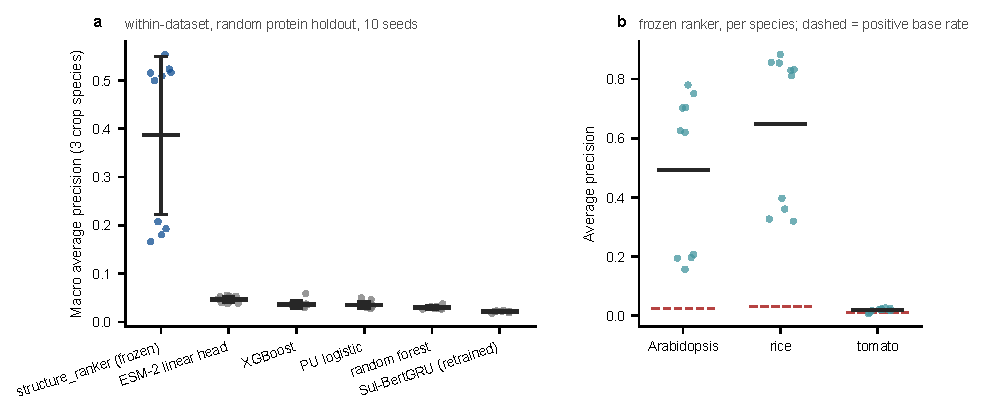
\includegraphics[width=\textwidth]{fig2_benchmark.pdf}}
\caption{Within-dataset literature-comparable benchmark.}
\label{fig:benchmark}
\end{figure}

\begin{figure}[!htbp]
\center{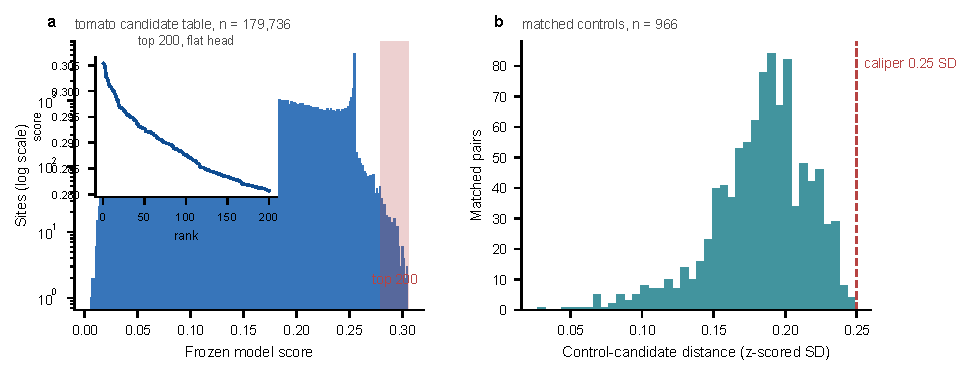
\includegraphics[width=\textwidth]{fig3_frozen_release.pdf}}
\caption{Frozen tomato candidate release.}
\label{fig:release}
\end{figure}

\begin{figure}[!htbp]
\center{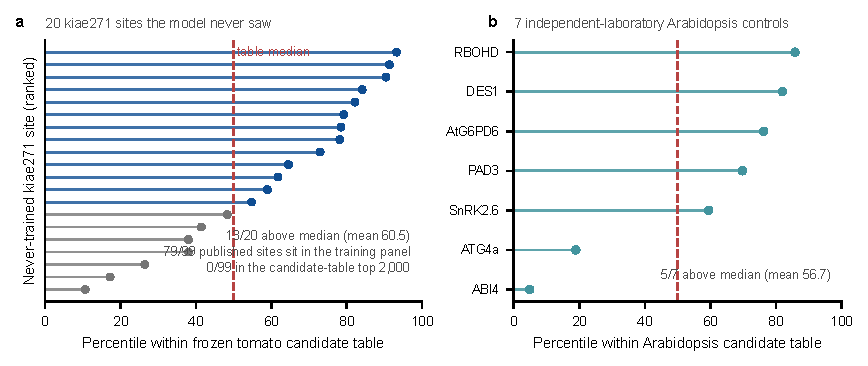
\includegraphics[width=\textwidth]{fig4_preblind_calibration.pdf}}
\caption{Pre-blind calibration against published sites.}
\label{fig:calibration}
\end{figure}

\begin{figure}[!htbp]
\center{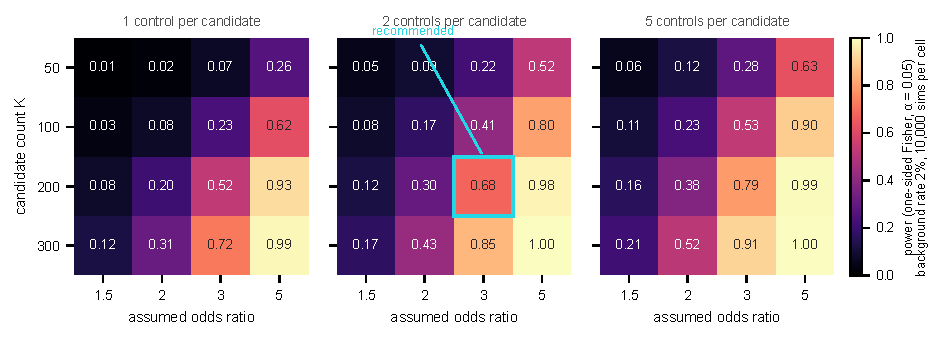
\includegraphics[width=\textwidth]{fig5_power_landscape.pdf}}
\caption{Preregistered power landscape.}
\label{fig:power}
\end{figure}

% [GATE 3 PLACEHOLDER] Figure 6 (blind-cohort result) is added after unblinding.
%\begin{figure}[!htbp]
%\center{\includegraphics[width=\textwidth]{fig6_blind_cohort.pdf}}
%\caption{Blind-cohort result.}
%\label{fig:blind}
%\end{figure}

\end{document}
